\section{Arrizak Furqona Gifary (1174070)}
\subsection{Teori}

\subsubsection{Binary Classification}
\begin{figure}[H]
\centerline{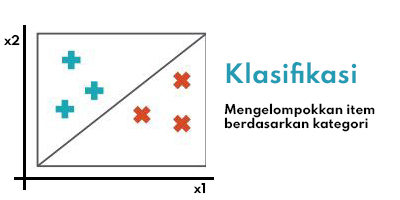
\includegraphics[width=10cm]{figures/1174070/2/1.jpg}}
\caption{Binary Classification}
\label{labelgambar}
\end{figure}
Binary Classification (Klasifikasi Biner) adalah sebuah tugas yang mengklasifikasikan elemen-elemen dari himpunan yang diberikan ke dalam dua kelompok (memprediksi kelompok mana yang masing-masing dimiliki) berdasarkan aturan klasifikasi. Konteks yang membutuhkan keputusan apakah suatu item memiliki sifat kualitatif atau tidak, beberapa karakteristik tertentu, atau beberapa klasifikasi
biner khas meliputi:
\begin{enumerate}
\item Tes medis 

untuk menentukan apakah pasien memiliki penyakit tertentu atau tidak - properti klasifikasi adalah keberadaan penyakit.

\item Metode uji ”lulus atau gagal”

Kontrol kualitas di pabrik, yaitu memutuskan apakah suatu spesifikasi telah atau belum terpenuhi - klasifikasi Go/no go.

\item Pengambilan informasi

memutuskan apakah suatu halaman atau artikel harus ada dalam hasil pencarian atau tidak - properti klasifikasi adalah relevansi artikel.
\end{enumerate}

\subsubsection{Supervised Learning , Unsupervised Learning dan Clusterring}

\begin{enumerate}
\item Supervised Learning

Supervised learning adalah suatu pembelajaran yang terawasi dimana jika output yang diharapkan telah diketahui sebelumnya. Biasanya pembelajaran ini dilakukan dengan menggunakan data yang telah ada.
Dan Supervised Learning dalam bahasa indonesia adalah pembelajaran yang ada supervisornya. Maksud disini ada supervisornya adalah label di tiap data nya. Label maksudnya adalah tag dari data yang ditambahkan dalam machine learning model. Contohnya gambar kucing di tag “kucing” di tiap masing masing image kucing dan gambar anjing di tag “anjing” di tiap masing gambar anjing.
\begin{figure}[H]
\centerline{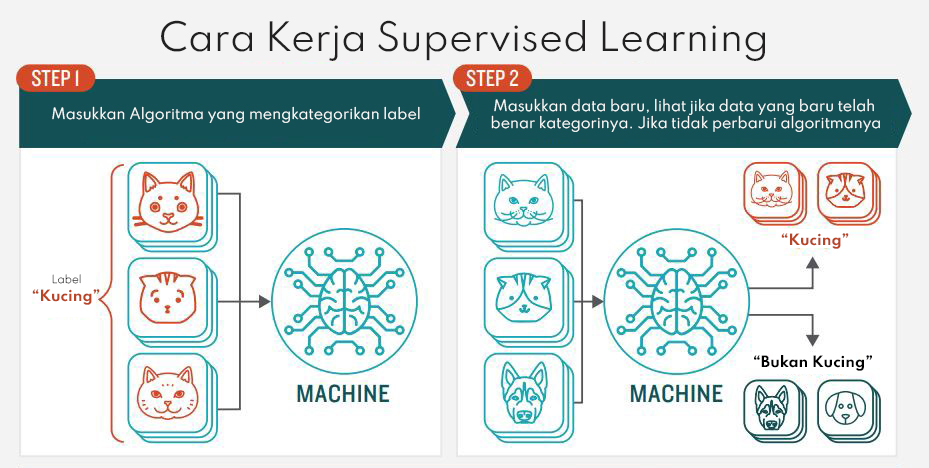
\includegraphics[width=10cm]{figures/1174070/2/2.jpg}}
\caption{Supervised Learning}
\label{labelgambar}
\end{figure}

\item Unsupervised Learning

Unsupervised learning menggunakan kemiripan dari attribut yang dimiliki suatu item. Jika attribut dan sifat dari data yang diekstrak memiliki kemiripan, maka akan dikelompokan (clustering). Sehingga hal ini akan menimbulkan kelompok (cluster). Jumlah cluster bisa unlimited. Dari kelompok-kelompok itu model dilabelkan, dan jika data baru mau di prediksi, maka akan dicocokkan dengan data kelompok yang mirip featurenya.
\begin{figure}[H]
\centerline{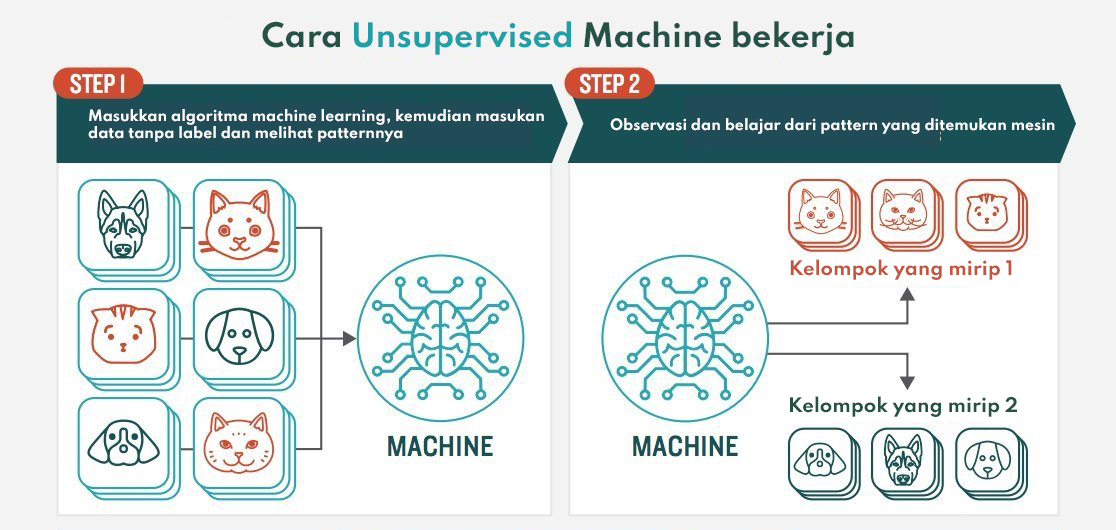
\includegraphics[width=10cm]{figures/1174070/2/3.jpg}}
\caption{Unsupervised Learning}
\label{labelgambar}
\end{figure}

\item Clusterring

Clustering adalah sebuah metode untuk membedakan data-data menjadi sebuah kumpulan dari group yang isinya merupakan data yang mirip setiap grupnya. Basisnya dapat berupa kesamaan atau perbedaan dari setiap grup tersebut.
\begin{figure}[H]
\centerline{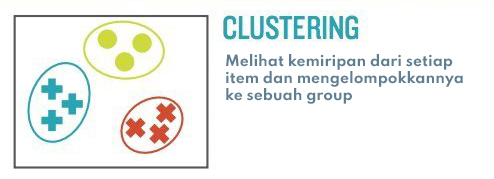
\includegraphics[width=10cm]{figures/1174070/2/4.jpg}}
\caption{Clusterring}
\label{labelgambar}
\end{figure}
\end{enumerate}

\subsubsection{Evaluasi dan Akurasi}

Evaluasi adalah tentang bagaimana kita dapat mengevaluasi seberapa baik model bekerja dengan mengukur tingkat akurasinya. Dan akurasi akan didefinisikan sebagai persentase kasus yang diklasifikasikan dengan benar. Kita dapat menganalisis kesalahan yang dibuat oleh model,atau tingkat kebingungannya, menggunakan matriks kebingungan(confusion matrix). Matriks kebingungan mengacu pada kebingungan dalam model,tetapi matriks kebingungan ini bisa menjadi sedikit sulit untuk dipahami ketika mereka menjadi sangat besar.
\begin{figure}[H]
\centerline{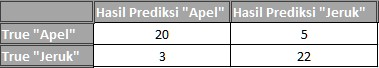
\includegraphics[width=10cm]{figures/1174070/2/5.jpg}}
\caption{Evaluasi}
\label{labelgambar}
\end{figure}

\subsubsection{Cara Membuat Confusion Matrix}

Confusion Matrix merupakan metode untuk menghitung akurasi pada data mining atau Sistem Pendukung Keputusan. Untuk menggunakan Confusion Matrix, ada 4 istilah sebagai hasil proses dari klasifikasi. Diantaranya adalah:
\begin{itemize}
\item True Positive: Data positif yang terdeteksi memiliki hasil benar
\item False Positive: Data Positif yang terdeteksi memiliki hasil salah
\item True Negative: Data negatif yang terdeteksi memiliki hasil benar
\item False Negative: Data negatif yang terdeteksi memiliki hasil salah
\end{itemize}
\begin{figure}[H]
\centerline{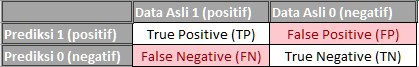
\includegraphics[width=10cm]{figures/1174070/2/6.jpg}}
\caption{Contoh Confusion Matrix}
\label{labelgambar}
\end{figure}

\subsubsection{Bagaimana K-fold cross validation bekerja}
\begin{enumerate}
\item Total instance dibagi menjadi N bagian.
\item Fold yang pertama adalah bagian pertama menjadi data uji (testing data) dan sisanya menjadi training data.
\item Lalu hitung akurasi berdasarkan porsi data tersebut dengan menggunakan persamaan.
\item Fold yang kedua adalah bagian kedua, yang menjadi data uji(testing data)dan sisanya training  data.
\item Kemudian hitung akurasi berdasarkan porsi data tersebut.
\item Dan seterusnya hingga habis mencapai fold ke-K.
\item Terakhir hitung rata-rata akurasi K buah.
\end{enumerate}
\begin{figure}[H]
\centerline{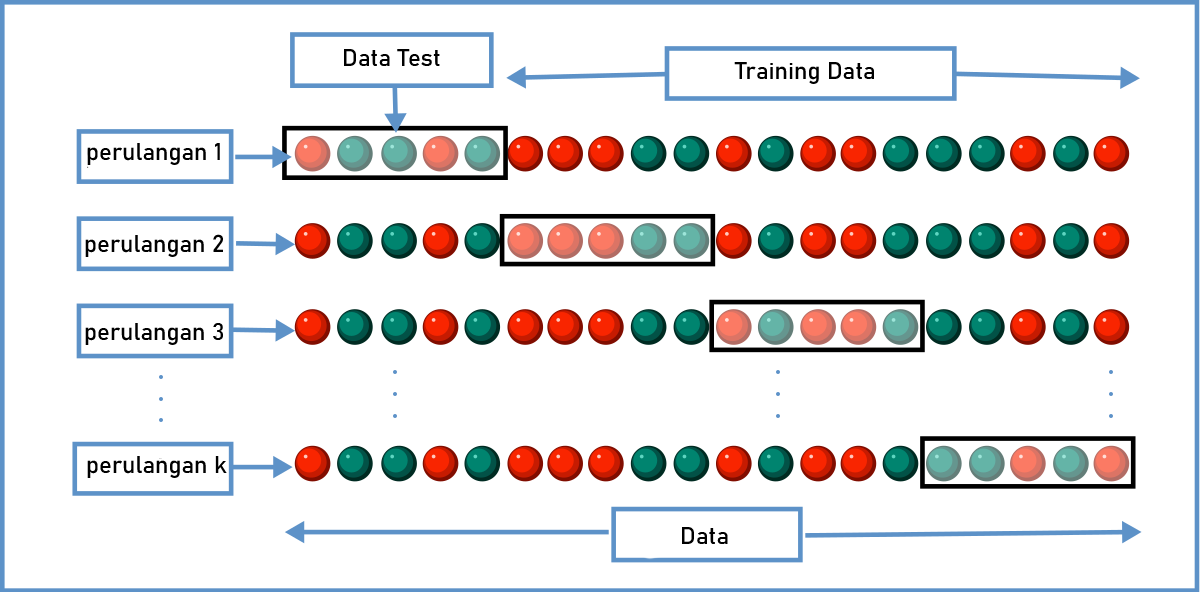
\includegraphics[width=10cm]{figures/1174070/2/7.png}}
\caption{Contoh K-Fold Cross Validation}
\label{labelgambar}
\end{figure}

\subsubsection{Apa itu Decision Tree}

Decision Tree adalah sebuah struktur yang menentukan keputusan dan setiap konsekuensinya. Hasil dari setiap struktur biasanya menggunakan jawaban (True dan False) atau cabang lain yang akan menjadi pohon selanjutnya. Setiap keputusan diantaranya akan membandingkan kondisi yang diberikan kepada struktur untuk dibandingkan kondisi apa saja yang sudah didapat pada sistem tersebut.
\begin{figure}[H]
\centerline{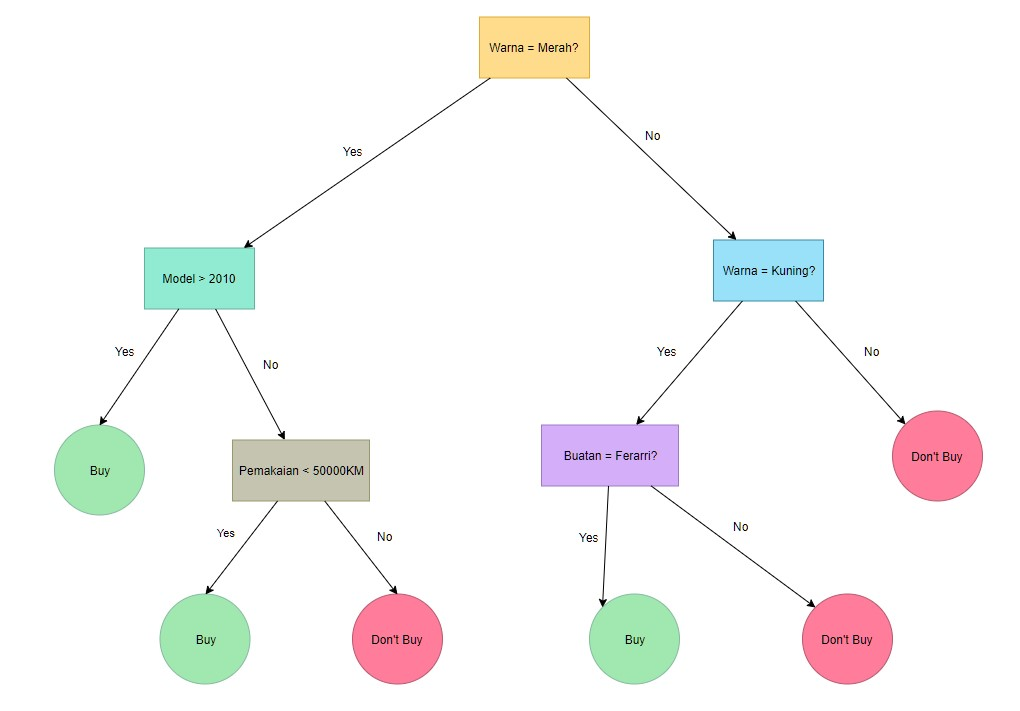
\includegraphics[width=10cm]{figures/1174070/2/8.jpg}}
\caption{Contoh Decision Tree membeli mobil}
\label{labelgambar}
\end{figure}

\subsubsection{Information Gain dan Entropi}
\begin{itemize}
\item Information Gain

Information Gain merupakan total data yang didapat dari data - data acak yang data tersebut akan digunakan untuk analisis data lainnya. Information Gain ini digunakan pada decision tree sebagai label setiap aksi - aksi yang perlu dinilai validasinya.
\begin{figure}[H]
\centerline{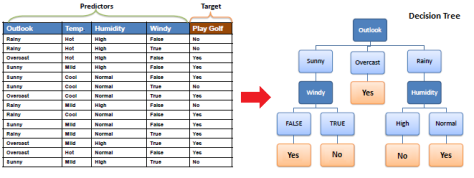
\includegraphics[width=10cm]{figures/1174070/2/9.png}}
\caption{Information Gain}
\label{labelgambar}
\end{figure}

\item Entropi

Entropi merupakan pengukuran sebuah data dan validnya data tersebut untuk dapat digunakan sebagai informasi yang akan dimasukkan ke Information Gain. Entropi menilai sebuah obyek berdasarkan kebutuhan di dunia nyata dan pengaruh pada sistem yang akan digunakan.
\begin{figure}[H]
\centerline{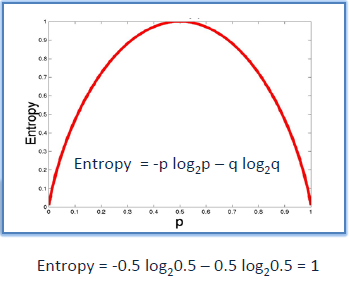
\includegraphics[width=10cm]{figures/1174070/2/10.png}}
\caption{Entropi}
\label{labelgambar}
\end{figure}
\end{itemize}


\subsection{Praktek}
Tugas anda adalah, dataset ganti menggunakan student-mat.csv dan mengganti semua nama variabel dari kode di bawah ini dengan nama-nama makanan (NPM mod 3=0), kota (NPM mod 3=1), buah (NPM mod 3=2)
\lstinputlisting[firstline=8, lastline=9]{src/1174070/2/1.py} 

\subsubsection{Nomor 1}
\hfill\\
\lstinputlisting[firstline=12, lastline=14]{src/1174070/2/1.py}
\begin{figure}[H]
\centerline{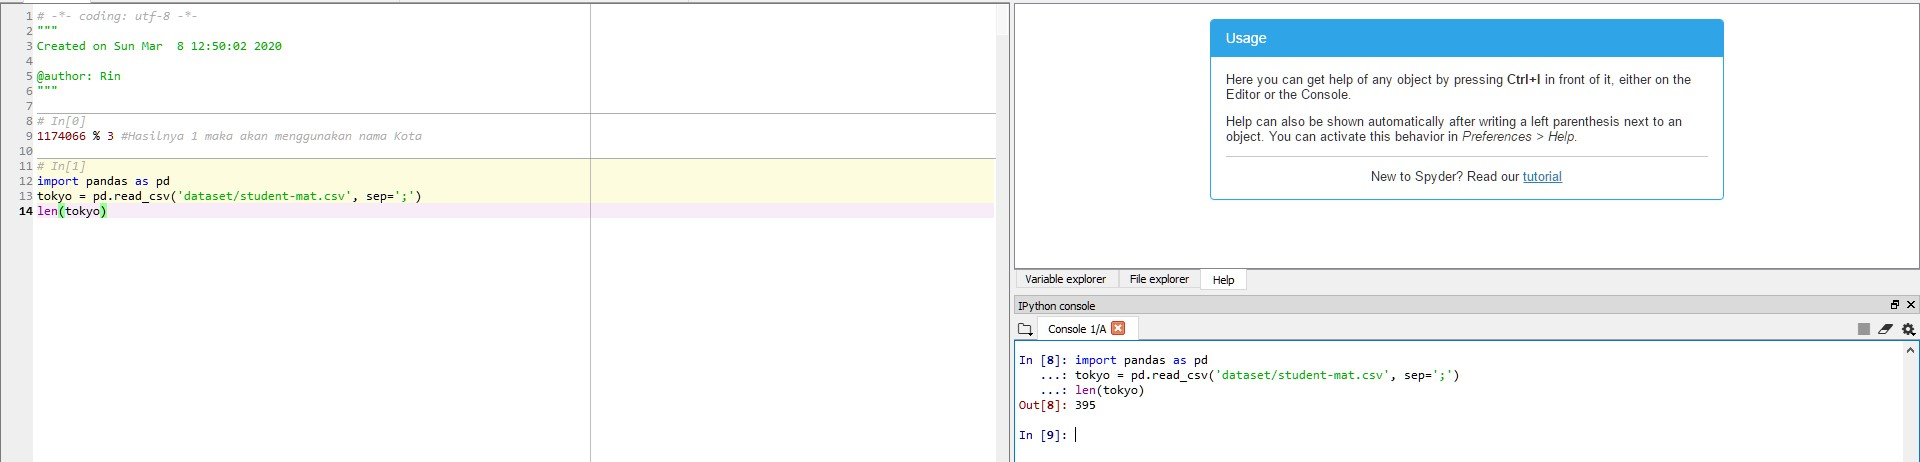
\includegraphics[width=10cm]{figures/1174070/2/11.jpg}}
\caption{Nomor 1}
\label{labelgambar}
\end{figure}

\subsubsection{Nomor 2}
\hfill\\
\lstinputlisting[firstline=16, lastline=20]{src/1174070/2/1.py}
\begin{figure}[H]
\centerline{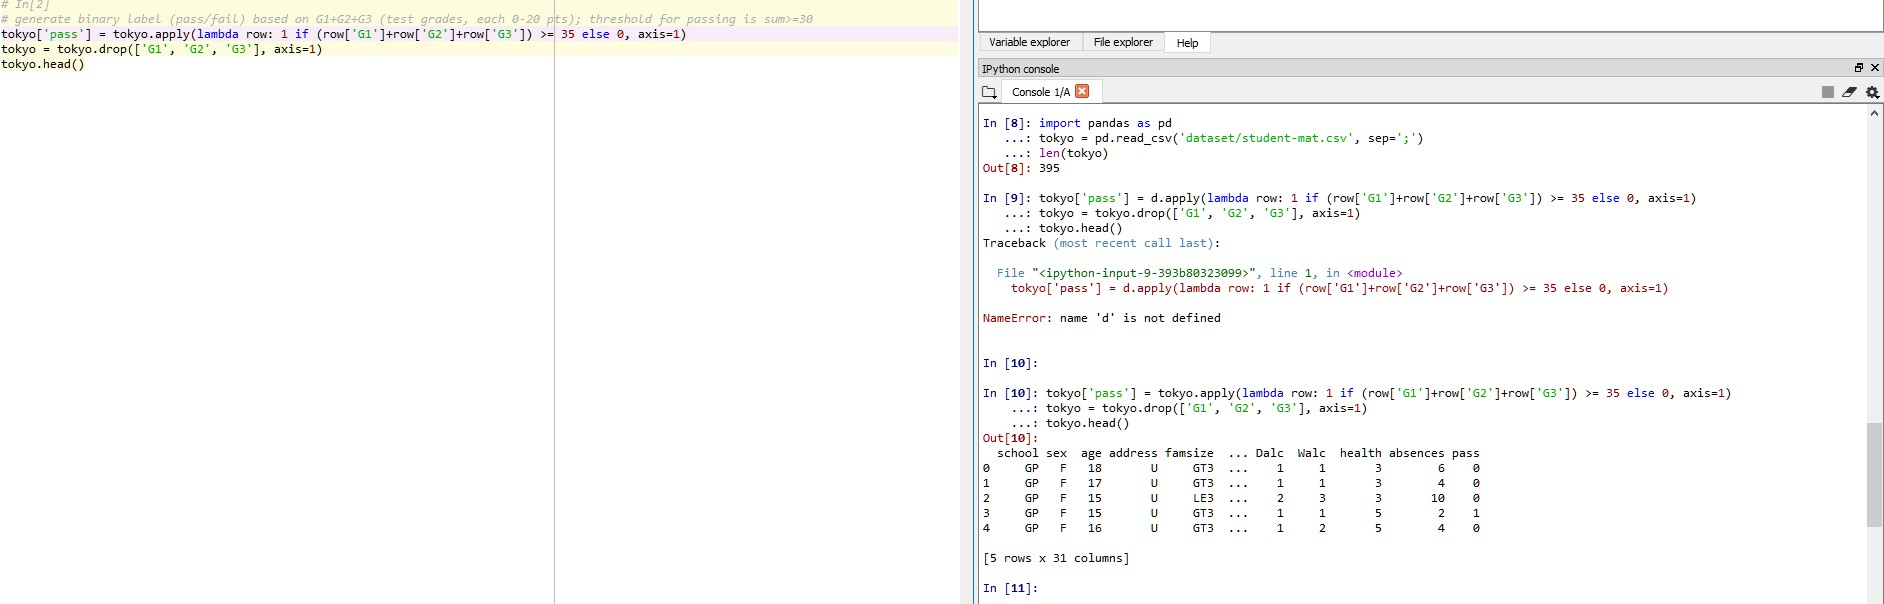
\includegraphics[width=10cm]{figures/1174070/2/12.jpg}}
\caption{Nomor 2}
\label{labelgambar}
\end{figure}

\subsubsection{Nomor 3}
\hfill\\
\lstinputlisting[firstline=22, lastline=27]{src/1174070/2/1.py}
\begin{figure}[H]
\centerline{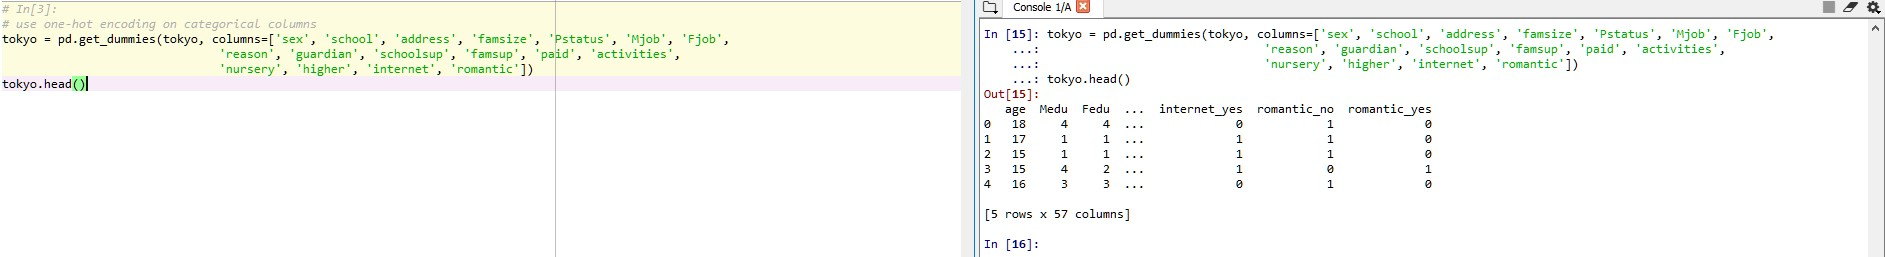
\includegraphics[width=10cm]{figures/1174070/2/13.jpg}}
\caption{Nomor 3}
\label{labelgambar}
\end{figure}

\subsubsection{Nomor 4}
\hfill\\
\lstinputlisting[firstline=29, lastline=47]{src/1174070/2/1.py}
\begin{figure}[H]
\centerline{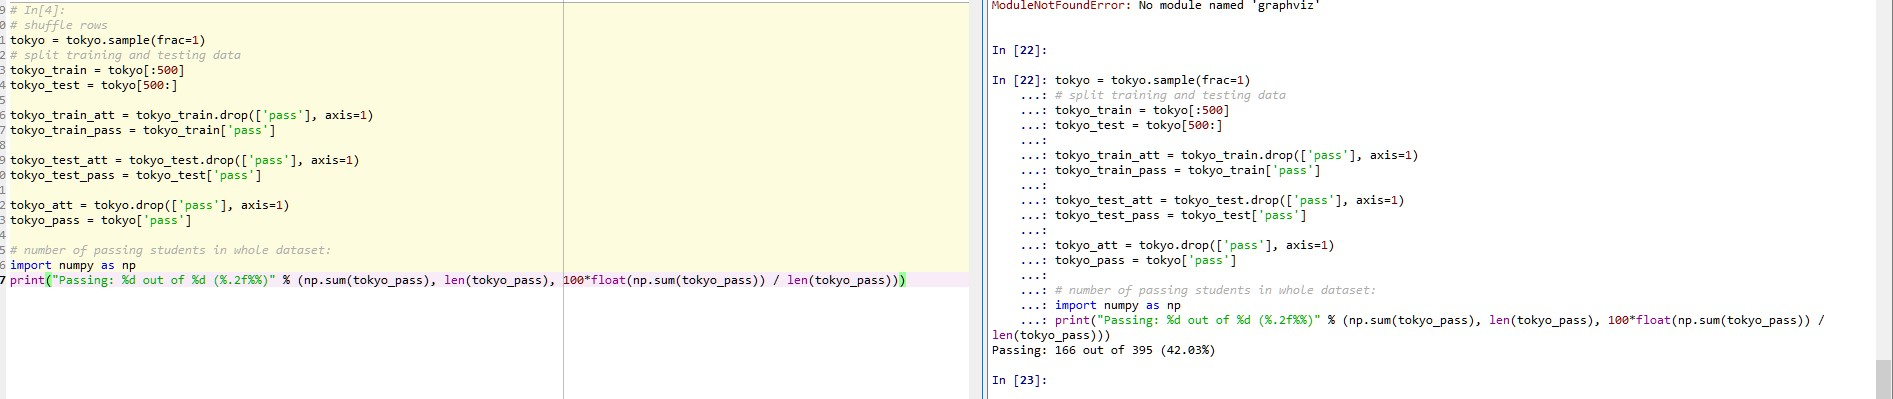
\includegraphics[width=10cm]{figures/1174070/2/14.jpg}}
\caption{Nomor 4}
\label{labelgambar}
\end{figure}

\subsubsection{Nomor 5}
\hfill\\
\lstinputlisting[firstline=49, lastline=53]{src/1174070/2/1.py}
\begin{figure}[H]
\centerline{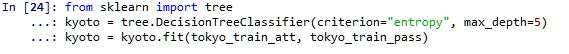
\includegraphics[width=10cm]{figures/1174070/2/15.jpg}}
\caption{Nomor 5}
\label{labelgambar}
\end{figure}

\subsubsection{Nomor 6}
\hfill\\
\lstinputlisting[firstline=56, lastline=63]{src/1174070/2/1.py}
\begin{figure}[H]
\centerline{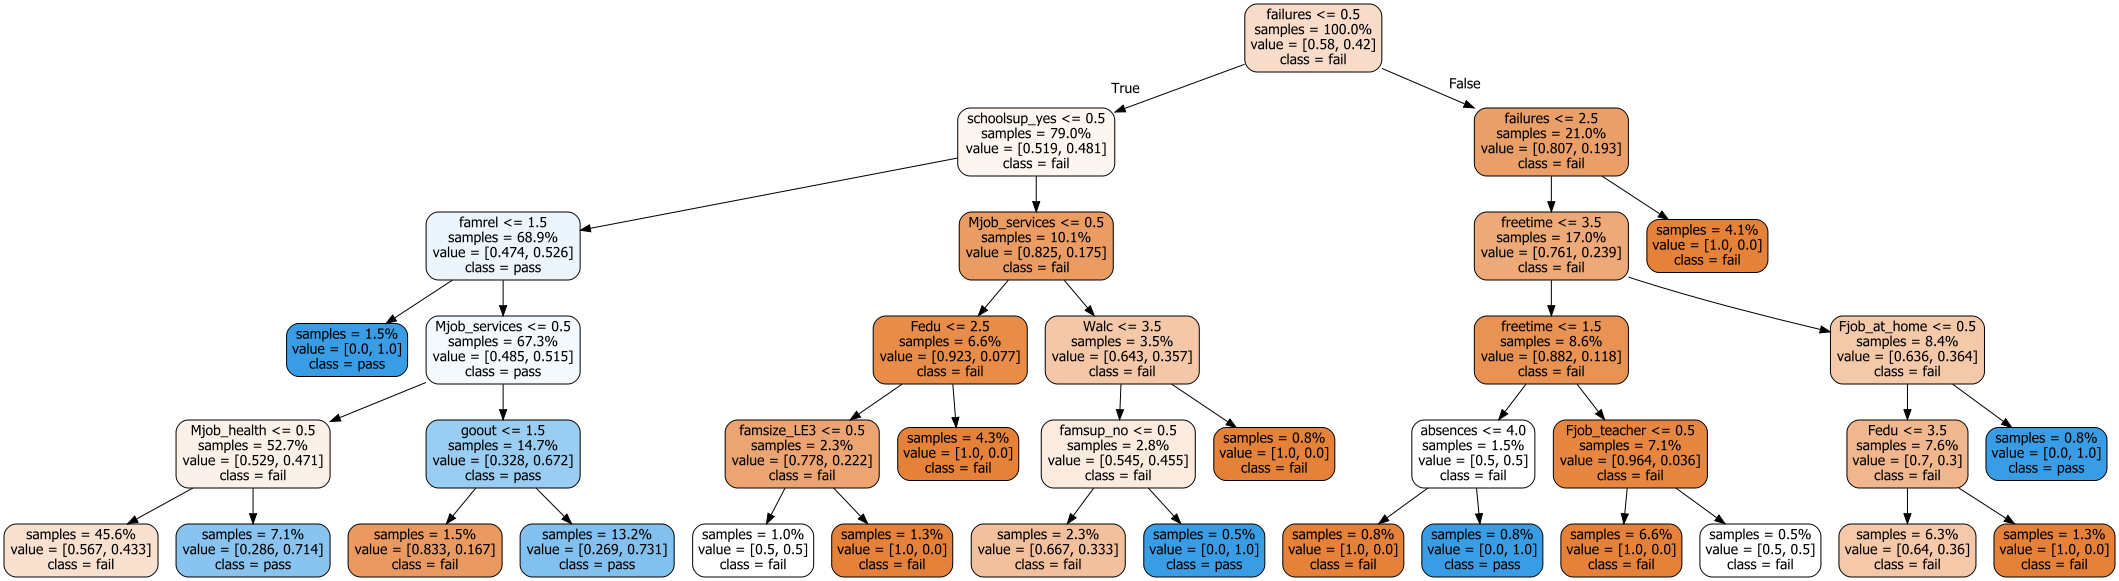
\includegraphics[width=10cm]{figures/1174070/2/16.png}}
\caption{Nomor 6}
\label{labelgambar}
\end{figure}

\subsubsection{Nomor 7}
\hfill\\
\lstinputlisting[firstline=66, lastline=70]{src/1174070/2/1.py}
\begin{figure}[H]
\centerline{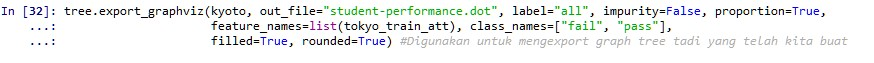
\includegraphics[width=10cm]{figures/1174070/2/17.jpg}}
\caption{Nomor 7}
\label{labelgambar}
\end{figure}

\subsubsection{Nomor 8}
\hfill\\
\lstinputlisting[firstline=73, lastline=74]{src/1174070/2/1.py}
\begin{figure}[H]
\centerline{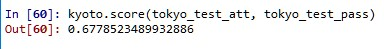
\includegraphics[width=10cm]{figures/1174070/2/18.jpg}}
\caption{Nomor 8}
\label{labelgambar}
\end{figure}

\subsubsection{Nomor 9}
\hfill\\
\lstinputlisting[firstline=77, lastline=81]{src/1174070/2/1.py}
\begin{figure}[H]
\centerline{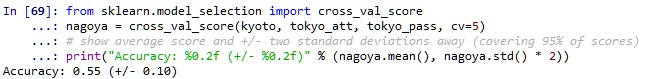
\includegraphics[width=10cm]{figures/1174070/2/19.jpg}}
\caption{Nomor 9}
\label{labelgambar}
\end{figure}

\subsubsection{Nomor 10}
\hfill\\
\lstinputlisting[firstline=84, lastline=88]{src/1174070/2/1.py}
\begin{figure}[H]
\centerline{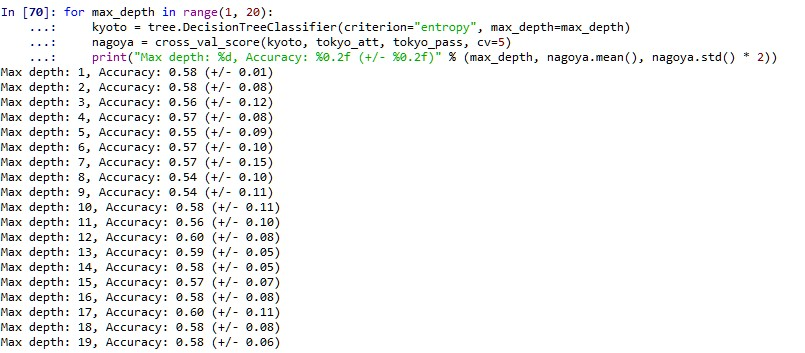
\includegraphics[width=10cm]{figures/1174070/2/20.jpg}}
\caption{Nomor 10}
\label{labelgambar}
\end{figure}

\subsubsection{Nomor 11}
\hfill\\
\lstinputlisting[firstline=91, lastline=102]{src/1174070/2/1.py}
\begin{figure}[H]
\centerline{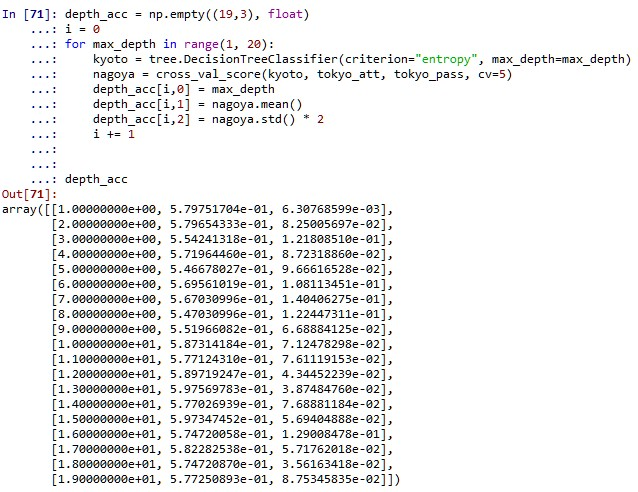
\includegraphics[width=10cm]{figures/1174070/2/21.jpg}}
\caption{Nomor 11}
\label{labelgambar}
\end{figure}

\subsubsection{Nomor 12}
\hfill\\
\lstinputlisting[firstline=105, lastline=109]{src/1174070/2/1.py}
\begin{figure}[H]
\centerline{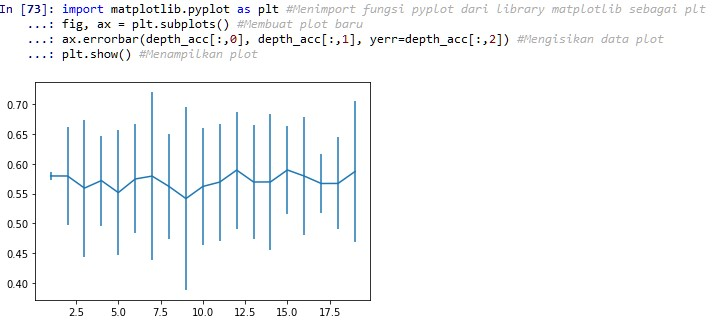
\includegraphics[width=10cm]{figures/1174070/2/22.jpg}}
\caption{Nomor 12}
\label{labelgambar}
\end{figure}

\subsection{Penanganan Error}
\subsubsection{Error}
\hfill\\
\begin{enumerate}
\item ModuleNotFoundError

\begin{figure}[H]
\centerline{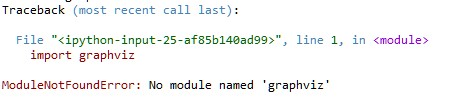
\includegraphics[width=10cm]{figures/1174070/2/error1.jpg}}
\caption{ModuleNotFoundError}
\label{labelgambar}
\end{figure}
\end{enumerate}

\subsubsection{Solusi}
\begin{enumerate}
\item Intall library Graphviz dengan cara download graphviz di google

setelah instalasi buka anaconda prompt sebagai admin lalu mengetikkan
\begin{lstlisting}
conda install graphviz
\end{lstlisting} 
\end{enumerate}

\subsection{Bukti Tidak Plagiat}
\hfill\\
\begin{figure}[H]
\centerline{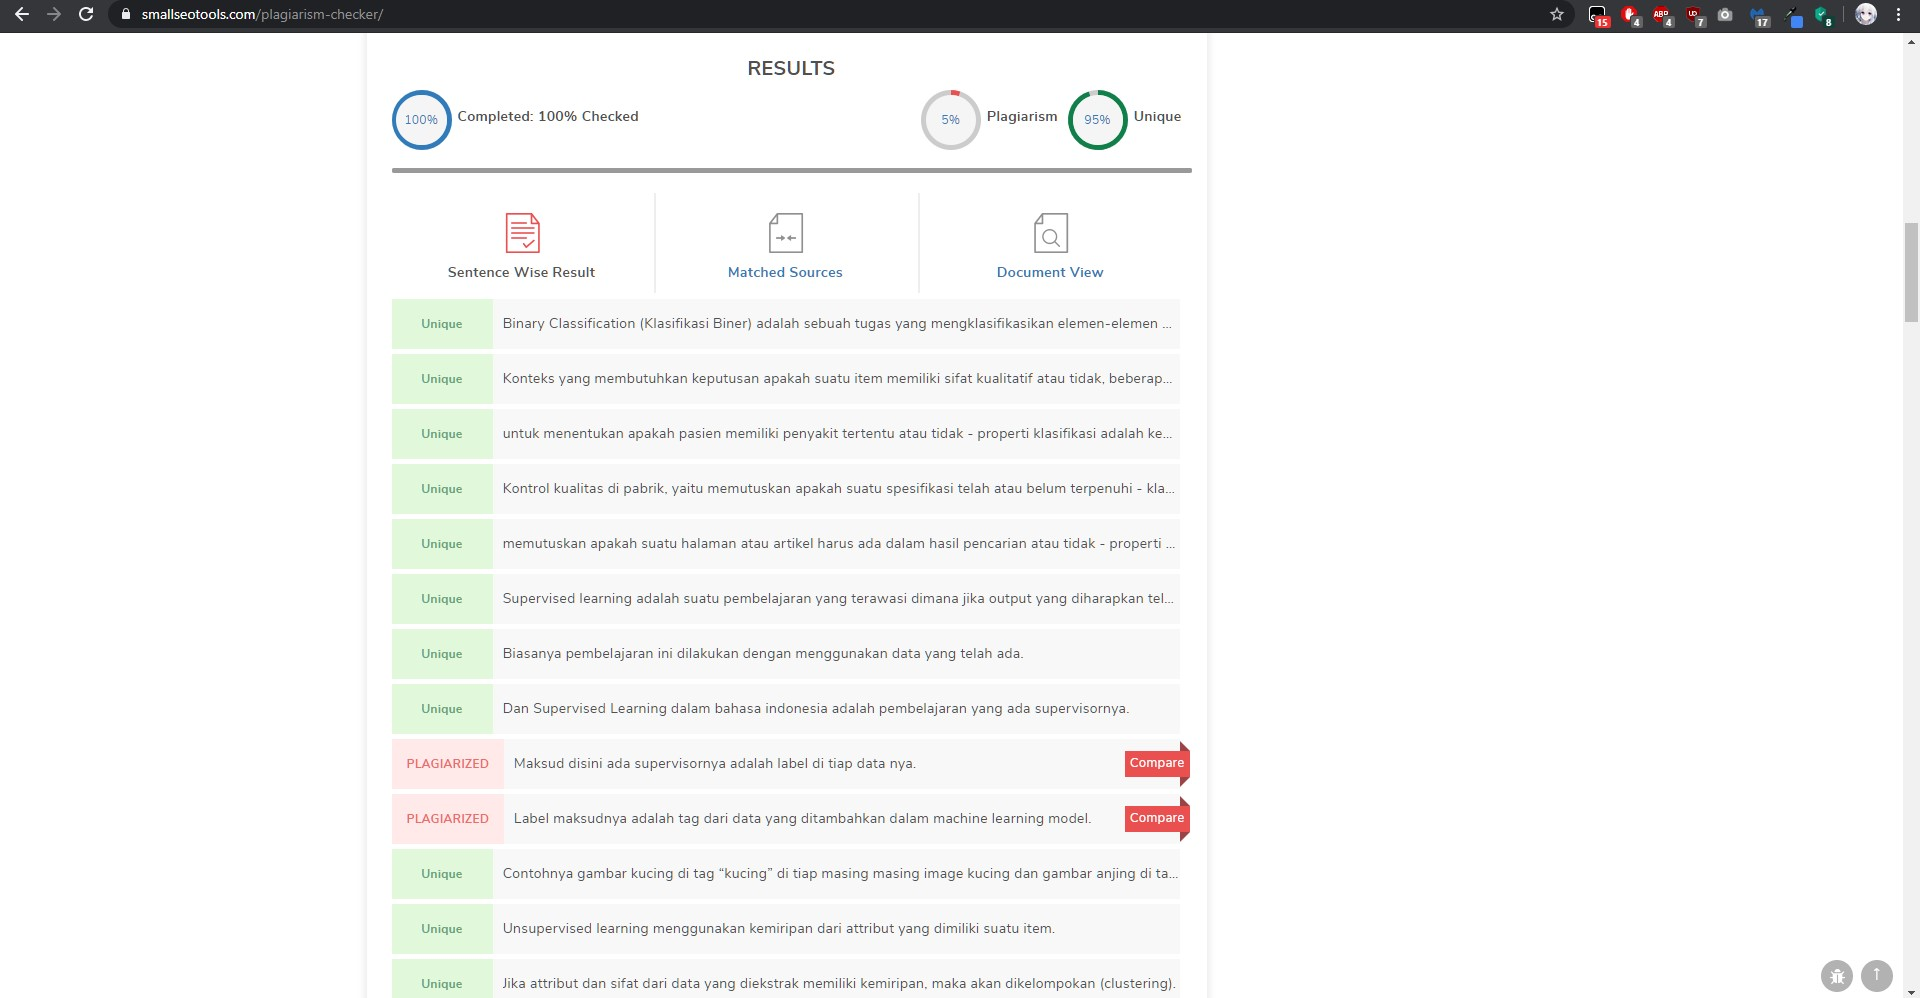
\includegraphics[width=10cm]{figures/1174070/2/plagiat.jpg}}
\caption{Bukti Tidak Plagiat}
\label{labelgambar}
\end{figure}

\subsection{Link Youtube:}
https://youtu.be/\_rB-Z2xMMdk